\documentclass{standalone}

\usepackage{tikz}
\usepackage{pgf-umlcd}
\usepackage[bitstream-charter]{mathdesign} % +1! taules mes petites i hi caben
\usepackage[T1]{fontenc}
\usepackage[utf8]{inputenc}

\begin{document}

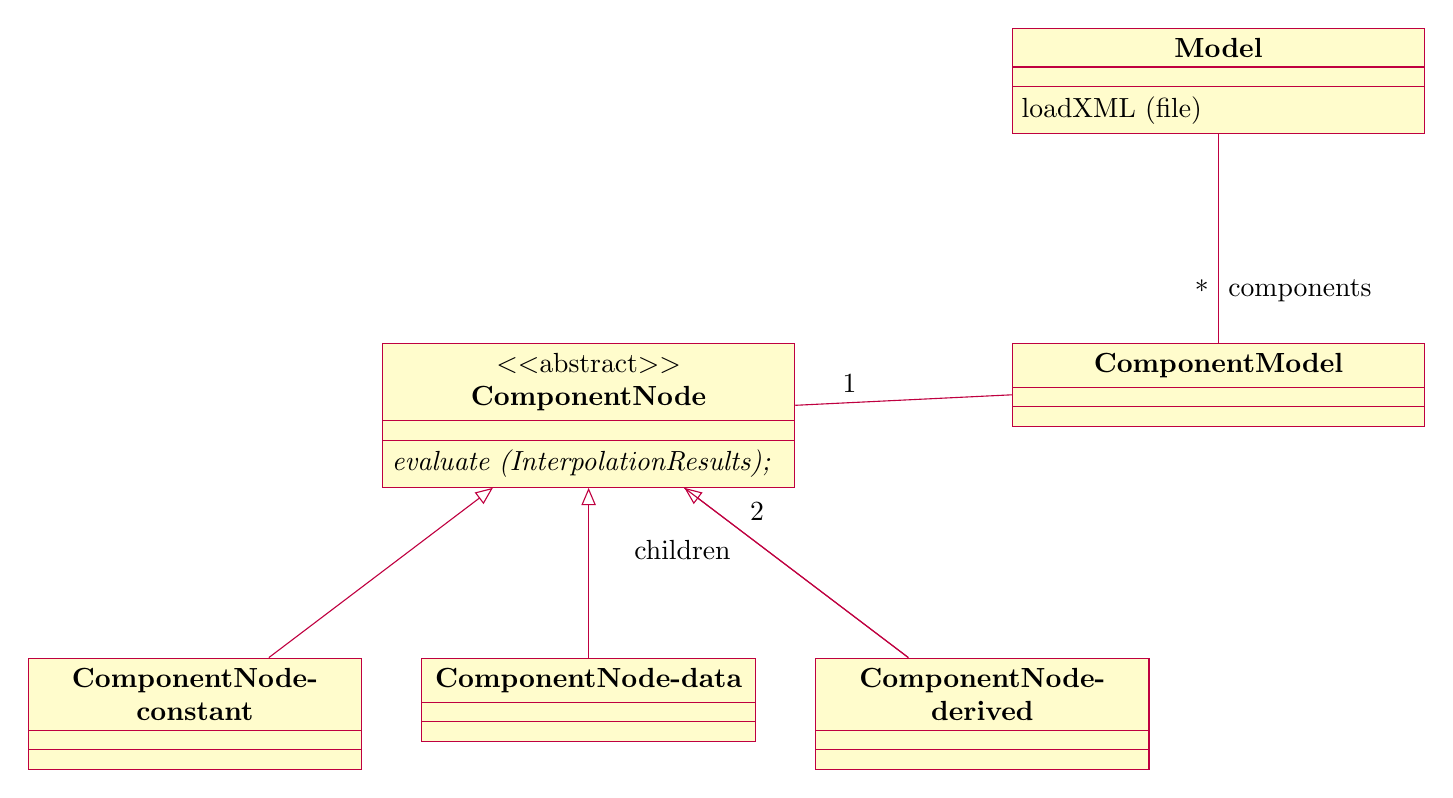
\begin{tikzpicture}

\begin{abstractclass}[text width=5cm]{ComponentNode}{0,0}
\operation[0]{evaluate (InterpolationResults);}
\end{abstractclass}

\begin{class}[text width=4cm]{ComponentNode-constant}{-5,-4}
\inherit{ComponentNode}
\end{class}
\begin{class}[text width=4cm]{ComponentNode-data}{0,-4}
\inherit{ComponentNode}
\end{class}
\begin{class}[text width=4cm]{ComponentNode-derived}{5,-4}
\inherit{ComponentNode}
\end{class}

\association{ComponentNode-derived}{}{}{ComponentNode}{children}{2};

\begin{class}[text width=5cm]{ComponentModel}{8,0}
\end{class}

\association{ComponentModel}{}{}{ComponentNode}{}{1}

\begin{class}[text width=5cm]{Model}{8,4}
\operation{loadXML (file)}
\end{class}

\association{Model}{}{}{ComponentModel}{components}{*}

\end{tikzpicture}

\end{document}
